% \section{Data-dependent double descent in adversarial training}
% lucas
% \subsection{Data Matters for Double Descent in Adversarial Training}
% \label{sect:factor}

\subsection{Dependence of epoch-wise double descent in adversarial training}
\label{sect:double-descent-adversarial}
\todo{Remove first two, already discussed in the main paper}

% \jingbo{I feel this section is a bit off-the-topic. It seems okay to totally skip this section and read the next two sections without confusion. Maybe move it to the appendix? }

% \chengyu{put this before the theoretical proof of dependence or after?}
% \lucas{current order is good. I changed titles.}

% \chengyu{Present as a validation of the theory, merged to there, only leave the figure}
% \chengyu{maybe keep the reconcile part (double descent behvaviours), but move this part to appendix. (this part can be an empirical verification of the next section)}

% We study the properties of double descent in adversarial training and find that it is conditioned on the perturbation radius and data quality.
% As larger model capacity and longer training can both increase the model complexity, double descent can occur in terms of model capacity and training epochs~\citep{Nakkiran2020DeepDD}. 
% \jingbo{I'm not very sure if we want to keep the model-wise double descent discussion here or move it to appendix. It is slightly off-topic given all the later discussions are focused on the epoch-wise one.}
% Therefore, we explore the model-wise double descent and epoch-wise double descent in adversarial training simultaneously and show that they are both conditioned on the data. Specifically, the magnitude of the double descent is controlled by the radius of the adversarial perturbation and the quality of the data.
% minimum distance to the (optimal?) decision boundary in the dataset. 
% The model-wise double descent and the epoch-wise double descent are both mitigated with small perturbation radius and high data quality.

% In this section, we show that the double descent in adversarial training is conditioned on the data quality. 
% As models are trained on adversarial examples, data properties in adversarial training are concerned with the quality of the clean examples, and the adversary employed to generate the perturbation, which further depends on the perturbation radius and the number of attack iterations\footnote{The best step size in terms of the model performance can often be determined from the combination of perturbation radius and attack iterations~\citep{Madry2018TowardsDL}}. We show that the double descent in adversarial training has a strong dependence on the data quality and the perturbation radius, but almost no dependence on the number of attack iterations.


% \smallsection{Perturbation radius}
% Overfitting has been shown to dominate in adversarial training, but rarely appear in standard training~\citep{Rice2020OverfittingIA}. This suggests the overfitting, or more generally double descent, is conditioned on the perturbation radius in adversarial training, since standard training and standard accuracy can be viewed as adversarial training and robust accuracy with zero perturbation radius, respectively. By modulating the perturbation radius, we show that such correlation is gradual.

% As shown in Figure \ref{fig:dependence-perturbation-quality}, the double descent emerges and exacerbates as the perturbation radius increases, indicating a strong correlation between perturbation radius and double descent in adversarial training. In particular, when the perturbation radius is around $4/255$, a second minimum can be observed which is equivalently good or even better than the first minimum. This again validates the strong connection between robust overfitting and double descent, and suggests longer training can still be helpful for adversarial training. % Note that when early stopping is employed, the model-wise double descent disappears, which is aligned with the observation in previous works~\citep{Nakkiran2020DeepDD, Rice2020OverfittingIA}.






% % ===============================================
% % \subsection{Distance to the boundary}
% \smallsection{Data quality}
% Previous works have shown that some datasets such as ImageNet~\citep{Deng2009ImageNetAL} may produce significantly stronger robust overfitting~\citep{Rice2020OverfittingIA}. It has also been observed that the low-quality data in the same dataset causes the robust overfitting~\citep{Dong2021DataPF}. 
% % We also empirically observe that adversarial training on MNIST~\citep{LeCun2005TheMD} incurs no robust overfitting (\chengyu{See Appendix for a discussion on the dataset}).
% This implies that the double descent in adversarial training hinges on the quality of the data. 
% % In this section, we show that in the same dataset, the double descent in adversarial training can be controlled by the the quality of the training data. % The double descent gradually dissipates as the quality of the data improves.
% % \chengyu{Maybe emphasize again this is not label noise}.
% We measure the data quality using the predictive probability of a classifier, and sample training sets with different levels of data quality controlled by a threshold of the quality-based rank.
% \todo{The sampled subset is restricted to class-balanced.}
% % , we rank the training examples based on their quality estimated above, and randomly sample a subset with a fixed size ($5\times 10^3$) from those examples above a specific threshold controlling the lowest quality. 
% Figure \ref{fig:dependence-perturbation-quality} shows that as the quality of the training set degrades, the double descent gradually emerges and exacerbates, indicating a strong correlation between the data quality and the double descent in adversarial training. One may again note that when the quality of the training data is relatively high, a second minimum can be observed which is equivalently good as the first minimum. 
% % \note{perturbation radius = 8/255, aligned with the default setting}

version https://git-lfs.github.com/spec/v1
oid sha256:122051f2431a5b436b094ebddc345f4fd484efcc0a36baa1a161ba0cc24b0baf
size 1294


% \smallsection{Dependence of double descent on the data quality}

% \begin{figure*}[!ht]
%   \centering
%   \includegraphics[width=0.9\textwidth]{figures/dependence-data.pdf}
%   \caption{Dependence of double descent on the data quality. As the quality of training data in adversarial training degrades, both the epoch-wise and model-wise double descent become more prominent. In the epoch-wise double descent figure, We smooth each curve by a window of 5 epochs to reduce the overlapping area. For the model-wise double descent the test error at the last checkpoint (solid line) and the test error at the best checkpoint (dashed line) are both shown. 
%   }
% \label{fig:dependence-data}
% \end{figure*}



% \chengyu{Need to run the experiments again}


% ===============================================
\smallsection{The number of attack iterations}
We have shown that the double descent in adversarial training strongly depends on the perturbation radius and the data quality. In this section we conduct experiments to show whether it also depends on the strength of the adversary. 
% A popular understanding of robust overfitting is the model overfits the adversarial perturbation as the inner maximization problem in adversarial training might not be sufficiently solved. However, in this section we modulate the strength of the adversary and show this is not the case.

In Figure~\ref{fig:dependence-iteration}, we fix the perturbation radius as $4/255$ where the double descent is relatively complete and vary the number of attack iterations of the PGD attack employed in the inner maximization. One may find that as long as the model capacity is reasonably large, the number of attack iterations will not significantly affect the double descent curve.
% , both for epoch-wise one and model-wise one. 
From the analysis of implicit label noise, this is easy to understand as more attack iterations will not reduce the probability corresponding to the true label much more---it is widely observed more iterations in PGD attack only marginally increase the attack successful rate. Consequently, the distribution mismatch between the true label distribution and the assigned label distribution that induces the implicit label noise will not expand significantly.


% \todo{Remove model-wise}
\begin{figure*}[!ht]
  \centering
  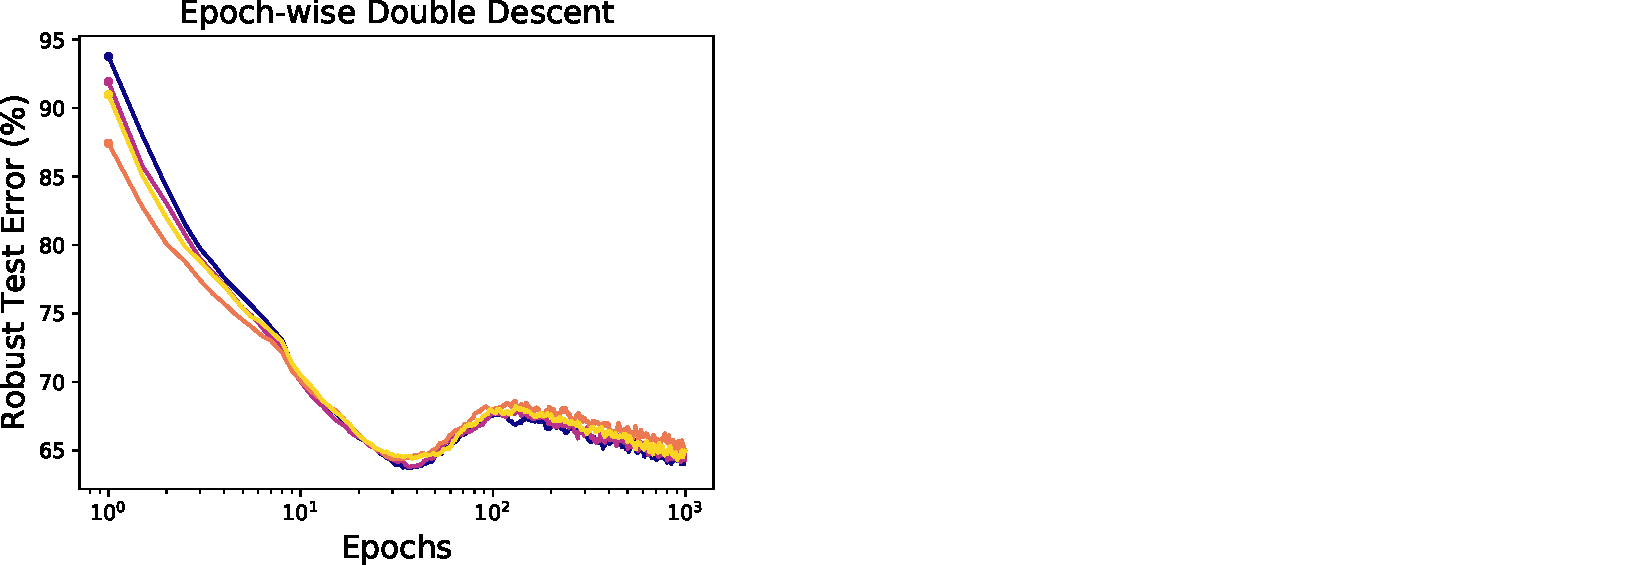
\includegraphics[width=0.45\textwidth]{figures/dependence-iteration.pdf}
  \caption{Dependence of epoch-wise double descent on the number of attack iterations. As more iterations are employed in the inner maximization, there is no significant change on epoch-wise double descent.
  }
\label{fig:dependence-iteration}
\end{figure*}

% \smallsection{Use AutoAttack for training}
% * AutoAttack is stronger than PGD-1000 (\cite{}).
% * Due to computation constraint, we adopt the regular training setting for this one.
% * An evidence showing that robust overfitting is not due to the model overfits weak perturbation (\cite{}?)
 

